\documentclass{article}
\usepackage{amsmath, amssymb, amsthm, graphicx}
\usepackage[export]{adjustbox}

\title{Chapter 2 Section 2}
\author{Andrew Taylor}
\date{April 6 2022}
\newtheorem{theorem}{Theorem}
\newtheorem{problem}{Problem}
\newtheorem*{solution}{Solution}
\DeclareMathOperator{\proj}{proj}
\DeclareMathOperator{\refl}{ref}
\newcommand{\vectorproj}[2][]{\proj_{#1}#2}
\newcommand{\vectorrefl}[2][]{\refl_{#1}#2}

\begin{document}
\maketitle

The letter L can be represented by the vectors $(0, 2)$ and $(1, 0)$. 

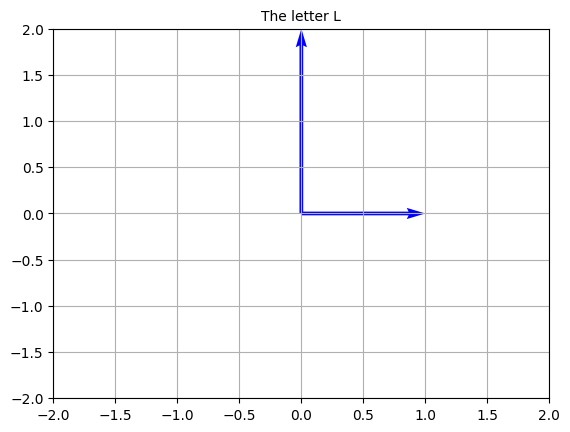
\includegraphics[scale=0.5, center]{L} 

The following problems ask for a linear transformation of the letter L. In the following problems, give the matrix of the transformation and plot the result.

\begin{problem}
Scale L by a factor of $\displaystyle \frac{1}{2}$
\end{problem}

\begin{solution}
The matrix of the transformation is 

\begin{align*}
\begin{bmatrix}
0.5 & 0.0 \\ 
0.0 & 0.5
\end{bmatrix}
\end{align*}

After the scaling, the L looks like this

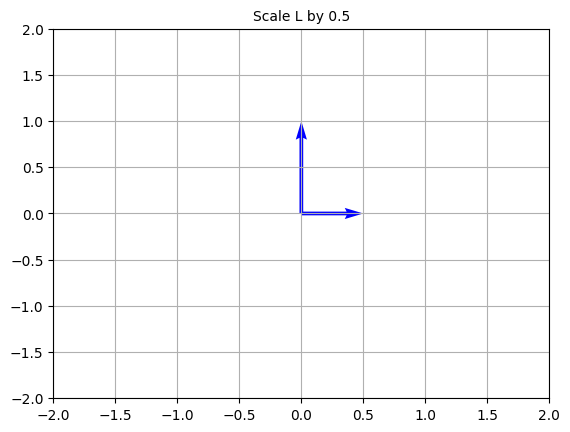
\includegraphics[scale=0.5, center]{Lscalebyhalf} 

Note that in creating this shape, we scaled both vectors that make up the L.

\end{solution}

\begin{problem}
Rotate L ninety degrees counterclockwise
\end{problem}

\begin{solution}
The matrix of the transformation is 

\begin{align*}
\begin{bmatrix}
0 & -1 \\ 
1 & 0
\end{bmatrix}
\end{align*}

After the rotation, the L looks like this

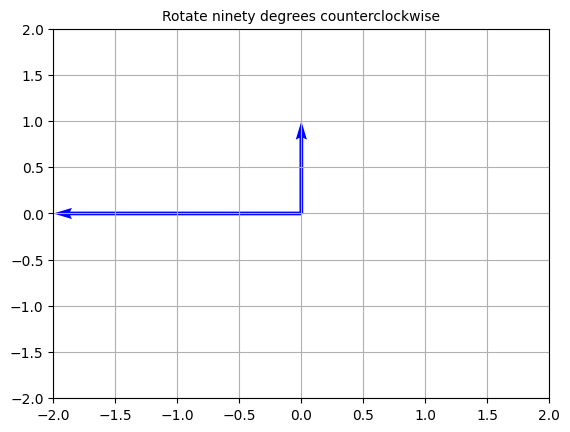
\includegraphics[scale=0.5, center]{Lrot90} 

\end{solution}

\begin{problem}
Reflect L about the Y axis
\end{problem}

\begin{solution}
The matrix of the transformation is

\begin{align*}
\begin{bmatrix}
-1 & 0 \\ 
0 & 1
\end{bmatrix}
\end{align*}

The plot looks like this

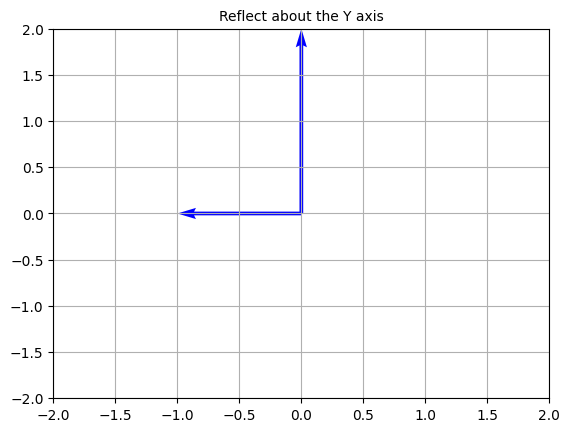
\includegraphics[scale=0.5, center]{Lreflecty} 

\end{solution}

\begin{problem}
Reflect L about the X axis
\end{problem}

\begin{solution}
The matrix of the transformation is 

\begin{align*}
\begin{bmatrix}
0 & 1 \\ 
-1 & 0
\end{bmatrix}
\end{align*}

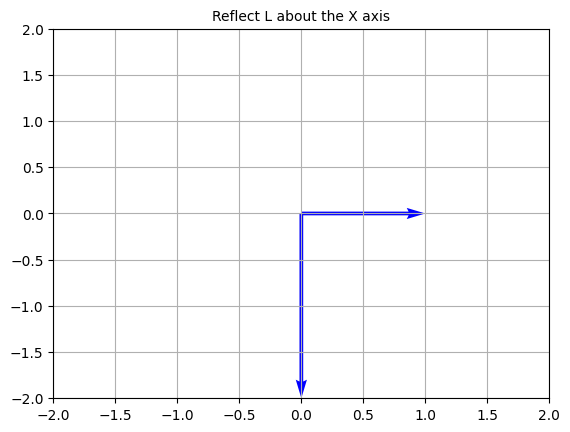
\includegraphics[scale=0.5, center]{Lreflectx} 

\end{solution}

\begin{problem}
Rotate L forty five degrees counterclockwise
\end{problem}

\begin{solution}
The matrix of the transformation is 

\begin{align*}
\begin{bmatrix}
\cos(\frac{\pi}{4}) & -1 * \sin(\frac{\pi}{4}) \\ 
\sin(\frac{\pi}{4}) & \cos(\frac{\pi}{4})
\end{bmatrix}
\end{align*}

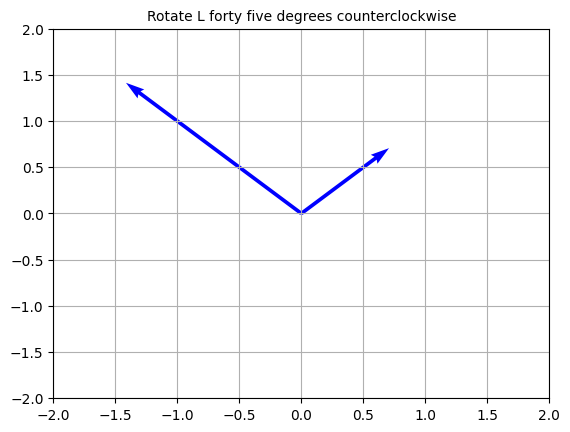
\includegraphics[scale=0.5, center]{Lrot45} 
\end{solution}

\begin{problem}
Find the orthogonal projection of L onto the x-axis
\end{problem}

\begin{solution}
The matrix of the transformation is 

\begin{align*}
\begin{bmatrix}
1 & 0 \\ 
0 & 0
\end{bmatrix}
\end{align*}

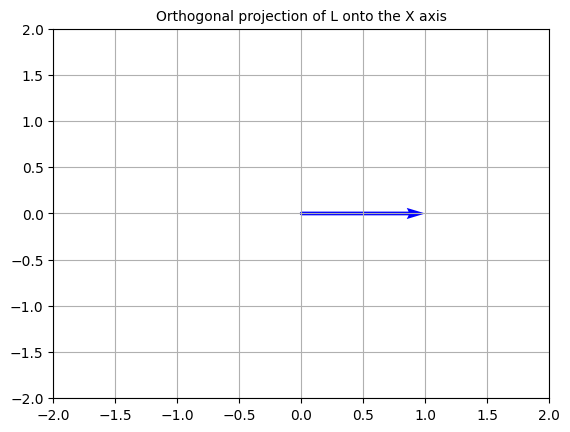
\includegraphics[scale=0.5, center]{Lorthogonalprojx} 

\end{solution}

\begin{problem}
Find the orthogonal projection of L onto the y-axis
\end{problem}

\begin{solution}
The matrix of the transformation is 

\begin{align*}
\begin{bmatrix}
0 & 0 \\ 
0 & 1
\end{bmatrix}
\end{align*}

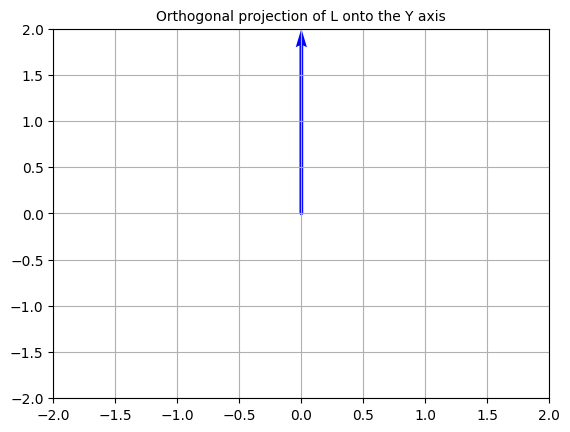
\includegraphics[scale=0.5, center]{Lorthogonalprojy} 

\end{solution}

\begin{problem}
Find the matrix P of the orthogonal projection onto the line L spanned by $\vec{w} = \begin{pmatrix} 3 \\ 4 \end{pmatrix}$
\end{problem}

\begin{solution}
\begin{align*}
P &= 
\displaystyle \frac{1}{w_{1}^2 + w_{2}^2} 
\begin{bmatrix}
w_{1}^2 & w_{1}w_{2} \\
w_{1}w_{2} & w_{2}^2
\end{bmatrix} \\
&=
\displaystyle \frac{1}{25} 
\begin{bmatrix}
9 & 12 \\
12 & 16
\end{bmatrix} \\
&= 
\begin{bmatrix}
0.36 & 0.48 \\
0.48 & 0.64
\end{bmatrix}
\end{align*}
\end{solution}

\begin{problem}
Let V be the plane defined by $2x_{1} + x_{2} - 2x_{3} = 0$ and let $\vec{x} = \begin{bmatrix}5 \\ 4 \\ -2 \end{bmatrix}$. Find $\vectorrefl[V]{\vec{x}}$.
\end{problem}

\begin{solution}
The vector $\vec{v} = \begin{bmatrix} 2 \\ 1 \\ -2 \end{bmatrix}$ is perpendicular to the plane V. 
\\
\\
We can get the unit vector $\vec{u}$ perpendicular to the plane by

\begin{align*}
\displaystyle \vec{u} &= \frac{1}{\Vert \vec{v} \rVert} \vec{v} \\
&= \displaystyle \frac{1}{\sqrt{2^2 + 1^2 + (-2)^2}} \begin{bmatrix} 2 \\ 1 \\ -2 \end{bmatrix} \\
&= \displaystyle \frac{1}{3} \begin{bmatrix} 2 \\ 1 \\ -2 \end{bmatrix} 
\end{align*}

We can now use the formula

\begin{align*}
\vectorrefl[V]{\vec{x}} &= \vectorproj[V]{\vec{x}} - \vectorproj[L]{\vec{x}} \\
&= \vec{x} - 2\vectorproj[L]{\vec{x}} \\
&= \vec{x} - 2(\vec{x} \cdot \vec{u}) \vec{u} \\
&= \begin{bmatrix} 5 \\ 4 \\ -2 \end{bmatrix} - 2\left(\begin{bmatrix} 5 \\ 4 \\ -2 \end{bmatrix} \cdot \frac{1}{3} \begin{bmatrix} 2 \\ 1 \\ -2 \end{bmatrix}\right) \frac{1}{3} \begin{bmatrix} 2 \\ 1 \\ -2 \end{bmatrix} \\
&= \begin{bmatrix} 5 \\ 4 \\ -2 \end{bmatrix} - 4 \begin{bmatrix} 2 \\ 1 \\ -2 \end{bmatrix} \\
&= \begin{bmatrix} 5 \\ 4 \\ -2 \end{bmatrix} - \begin{bmatrix} 8 \\ 4 \\ -8 \end{bmatrix} \\
&= \begin{bmatrix} -3 \\ 0 \\ 6 \end{bmatrix} 
\end{align*}

The reflection of the vector $\vec{x}$ over the plane V is the vector

\begin{align*}
\vectorrefl[V]\vec{x} = \begin{bmatrix} -3 \\ 0 \\ 6 \end{bmatrix} 
\end{align*}
\end{solution}

\begin{problem}
Give the matrix of a counterclockwise rotation through $\displaystyle \frac{\pi}{6}$.
\end{problem}

\begin{solution}
The matrix of a counterclockwise rotation through $\displaystyle \frac{\pi}{6}$ is

\begin{align*}
& \begin{bmatrix}
\cos\left(\displaystyle \frac{\pi}{6}\right) & -\sin\left(\displaystyle \frac{\pi}{6}\right) \\ \\
\sin\left(\displaystyle \frac{\pi}{6}\right) & \cos\left(\displaystyle \frac{\pi}{6}\right)
\end{bmatrix} \\ \\
&=
\begin{bmatrix}
\displaystyle \frac{\sqrt{3}}{2} & -\displaystyle \frac{1}{2} \\ \\
\displaystyle \frac{1}{2} & \displaystyle \frac{\sqrt{3}}{2}
\end{bmatrix} 
\end{align*}
\end{solution}

\begin{problem}
Let $T(\vec{x})$ be the linear transformation

\begin{align*}
T(\vec{x}) &= \begin{bmatrix}a & -b \\ b & a \end{bmatrix} \vec{x} \\
		&= \begin{bmatrix}a & -b \\ b & a \end{bmatrix} \begin{bmatrix} x_{1} \\ x_{2} \end{bmatrix}
\end{align*}

How does the linear transformation $T(\vec{x})$ affect the letter L? Remember that our letter L is composed of vectors $\begin{bmatrix} 0 \\ 2 \end{bmatrix}$ and $\begin{bmatrix} 1 \\ 0 \end{bmatrix}$.
\end{problem}

\begin{solution}
The vector $\begin{bmatrix} a \\ b \end{bmatrix}$ can be written in polar coordinates as

\begin{align*}
\begin{bmatrix} a \\ b \end{bmatrix} &= \begin{bmatrix} r \cos(\theta) \\ r \sin(\theta) \end{bmatrix}
\end{align*}

We can substitute these polar coordinates into the linear transformation, and write it as

\begin{align*}
T(\vec{x}) &= \begin{bmatrix}a & -b \\ b & a \end{bmatrix} \begin{bmatrix} x_{1} \\ x_{2} \end{bmatrix} \\
		&= \begin{bmatrix}r \cos(\theta) & -r \sin(\theta) \\ r \sin(\theta) & r \cos(\theta) \end{bmatrix} \begin{bmatrix} x_{1} \\ x_{2} \end{bmatrix} \\
		&= r \begin{bmatrix} \cos(\theta) & -\sin(\theta) \\ \sin(\theta) & \cos(\theta) \end{bmatrix} \begin{bmatrix} x_{1} \\ x_{2} \end{bmatrix} 
\end{align*}

The linear transformation rotates the vector counterclockwise through an angle of $\theta$ and scales the vector by a factor of $r$. 
\\ 
\\
For example, let $\begin{bmatrix} a \\ b \end{bmatrix} = \begin{bmatrix} 3 \\ 4 \end{bmatrix}$. Then we have

\begin{align*}
T(\vec{x}) &= \begin{bmatrix}3 & -4 \\ 4 & 3 \end{bmatrix} \begin{bmatrix} x_{1} \\ x_{2} \end{bmatrix} \\
		&\approx 5 \begin{bmatrix} \cos(53.1^\circ) & -\sin(53.1^\circ) \\ \sin(53.1^\circ) & \cos(53.1^\circ) \end{bmatrix} \begin{bmatrix} x_{1} \\ x_{2} \end{bmatrix} 
\end{align*}

This rotates L approximately $53.1^\circ$ and scales L by a factor of $5$.

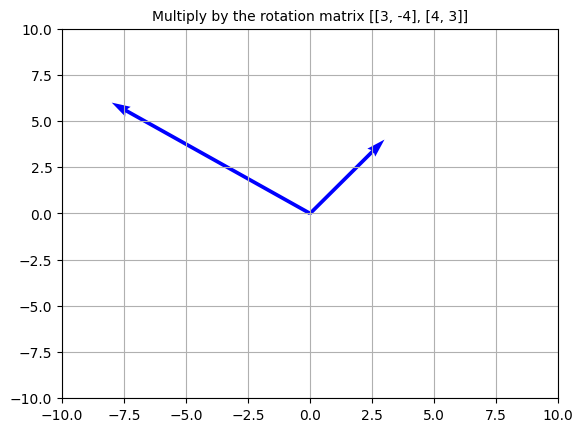
\includegraphics[scale=0.5, center]{Lrotscale345} 

Thus we see that the linear transformation

\begin{align*}
T(\vec{x}) &= \begin{bmatrix}a & -b \\ b & a \end{bmatrix} \begin{bmatrix} x_{1} \\ x_{2} \end{bmatrix} \\
		&= r \begin{bmatrix} \cos(\theta) & -\sin(\theta) \\ \sin(\theta) & \cos(\theta) \end{bmatrix} \begin{bmatrix} x_{1} \\ x_{2} \end{bmatrix} 
\end{align*}

rotates L counterclockwise through $\theta$ degrees and scales L by a factor of $r$.

\end{solution}

\begin{problem}
Sketch the image of the standard L under the linear transformation 

\begin{align*}
T(\vec{x}) = \begin{bmatrix} 3 & 1 \\ 1 & 2 \end{bmatrix} \vec{x}
\end{align*}
\end{problem}

\begin{solution}
We can apply the linear transformation to both vectors $\begin{bmatrix} 1 \\ 0 \end{bmatrix}$ and $\begin{bmatrix} 0 \\ 2 \end{bmatrix}$ that make up our L.

\begin{align*}
T\left(\begin{bmatrix} 1 \\ 0 \end{bmatrix}\right) &= \begin{bmatrix} 3 & 1 \\ 1 & 2 \end{bmatrix} \begin{bmatrix} 1 \\ 0 \end{bmatrix} \\
&= \begin{bmatrix} 3 \\ 1 \end{bmatrix}
\end{align*}

\begin{align*}
T\left(\begin{bmatrix} 0 \\ 2 \end{bmatrix}\right) &= \begin{bmatrix} 3 & 1 \\ 1 & 2 \end{bmatrix} \begin{bmatrix} 0 \\ 2 \end{bmatrix} \\
&= \begin{bmatrix} 2 \\ 4 \end{bmatrix}
\end{align*}

We can now draw these vectors on the Cartesian plane.

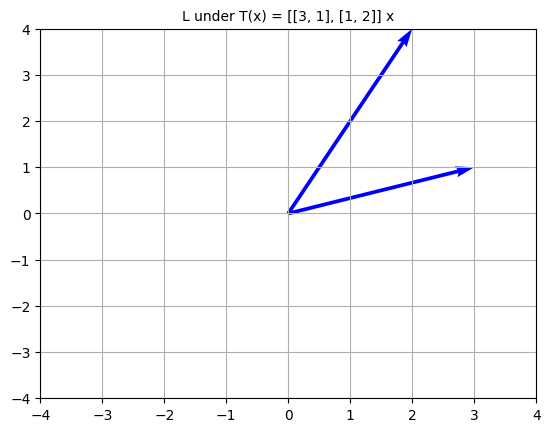
\includegraphics[scale=0.5, center]{L3112} 

\end{solution}

\begin{problem}
Find the matrix of a rotation through an angle of $60^\circ$ in the counterclockwise direction.
\end{problem}

\begin{solution}
The matrix of the rotation is

\begin{align*}
& \begin{bmatrix}
\cos(\frac{\pi}{3}) & -\sin(\frac{\pi}{3}) \\ \\
\sin(\frac{\pi}{3}) & \cos(\frac{\pi}{3})
\end{bmatrix} \\ \\
&= \begin{bmatrix}
\frac{1}{2} & -\frac{\sqrt{3}}{2} \\ \\
\frac{\sqrt{3}}{2}  & \frac{1}{2}
\end{bmatrix}
\end{align*}

\end{solution}

\begin{problem}
Consider a linear transformation from $\mathbb{R}^2$ to $\mathbb{R}^3$. Use $T(\vec{e_{1}})$ and $T(\vec{e_{2}})$ to describe the image of the unit square geometrically.
\end{problem}

\begin{solution}
Let $\vec{x}$ be a vector in the unit square. We can write the vector $\vec{x}$ as 

\begin{align*}
\vec{x} = x_{1} \vec{e_{1}} + x_{2} \vec{e_{2}}
\end{align*}
 
where $0 \leq x_{1}, x_{2} \leq 1$ and $\vec{e_{1}}$, $\vec{e_{2}}$ are the unit vectors. Thus

\begin{align*}
T(\vec{x}) &= T(x_{1} \vec{e_{1}} + x_{2} \vec{e_{2}}) \\\
&= T(x_{1} \vec{e_{1}}) + T(x_{2} \vec{e_{2}}) \\
&= x_{1} T(\vec{e_{1}}) + x_{2} T(\vec{e_{2}}) 
\end{align*}

The vectors $T(\vec{e_{1}})$ and $T(\vec{e_{2}})$ describe a parallelogram in $\mathbb{R}^3$. \\

Thus $T(\vec{x}) =  x_{1} T(\vec{e_{1}}) + x_{2} T(\vec{e_{2}})$ is a vector in that parallelogram in $\mathbb{R}^3$. \\

Note that we got our equation for $T(\vec{x})$ using the properties of linear transformations. \\

$T(a+b) = T(a) + T(b)$ and $T(ka)$ = $kT(a)$ for vectors $a, b$ and scalar $k$.
\end{solution} 

\begin{problem}
Interpret the following linear transformation geometrically:

\begin{align*}
T(\vec{x}) = \begin{bmatrix} 1 & 1 \\ -1 & 1 \end{bmatrix} \vec{x}
\end{align*}
\end{problem}

\begin{solution}
The matrix of the transformation is a rotation matrix combined with a scaling. Since a rotation matrix has the form 

\begin{align*}
\begin{bmatrix} a & -b \\ b & a \end{bmatrix}
\end{align*}

We see that $\begin{bmatrix} a \\ b \end{bmatrix} = \begin{bmatrix} 1 \\ -1 \end{bmatrix}$ \\ \\

The vector $\begin{bmatrix} 1 \\ -1 \end{bmatrix}$ forms a $-45^\circ$ angle with the X axis. The vector has magnitude $\sqrt{2}$. \\

Thus the linear transformation $T$ applies a rotation of $45^\circ$ in the clockwise direction and a scaling of $\sqrt{2}$.
\end{solution}

\begin{problem}
The matrix 

\begin{align*}
\begin{bmatrix}
-0.8 & -0.6 \\ 
0.6 & -0.8
\end{bmatrix}
\end{align*}

represents a rotation. Find the angle of rotation (in radians).
\end{problem}

\begin{solution}
We have $\begin{bmatrix} a \\ b \end{bmatrix} = \begin{bmatrix} -0.8 \\ 0.6 \end{bmatrix}$ and $a^2 + b^2 = 1$. \\

Thus $\cos(\theta) = -0.8$ and $\sin(\theta) = 0.6$ where $\theta$ is the angle of rotation. \\

We can solve for $\theta$.

\begin{align*}
& \cos(\theta) = -0.8 \\
& \theta = \cos^{-1}(-0.8) = 2.49809... 
\end{align*}

Thus $\theta \approx 2.49809$ radians.
\end{solution}

\end{document}